\documentclass[11pt]{article}
\usepackage{preamble}

\newcommand{\IconChart}{[CHART]}

\begin{document}

\packetheading{Lesson 4-3 \textperiodcentered\ Period 3 \textperiodcentered\ Student Packet}{Rational Expression Modeling + Assessment-Critical Simplify}

\sectionbanner{OBJECTIVES}
{\small
\renewcommand{\arraystretch}{1.25}
\noindent\begin{tabular}{|p{1.8in}|p{4.8in}|}
\hline
\textbf{Math Objective} & Model real-world ratios (surface area to volume, area ratios) as rational expressions; re-master simplification with domain restrictions on assessment-aligned items. \\ \hline
\textbf{Language Objective} & Interpret a simplified rational model in context, naming what \(x\), the numerator, and the denominator each represent. \\ \hline
\textbf{Essential Understanding} & The same simplify-and-restrict procedure handles both abstract and modeling problems --- units and context never change the math, only the interpretation. \\ \hline
\end{tabular}
}

\sectionbanner{TOPIC GOALS / ESSENTIAL QUESTION / MATERIALS}
{\small
\renewcommand{\arraystretch}{1.25}
\noindent\begin{tabular}{|p{1.8in}|p{4.8in}|}
\hline
\textbf{Topic Goals} & Simplify rational expressions with explicit domain restrictions (assessment-critical); model ratios of geometric quantities. \\ \hline
\textbf{Essential Question} & How do simplified rational expressions help us compare or scale real-world ratios, and what domain values are never allowed? \\ \hline
\textbf{Materials} & Student packet, pencil. Teacher pairs Example 2 (simplify) with Example 6 (SA/V) in Launch. Practice \#19 is the assessment rehearsal item --- Topic 4 LEHS Q\#2. \\ \hline
\end{tabular}
}

\sectionbanner{LAUNCH --- Simplify + Modeling (teacher models Ex 2 + Ex 6)}

\begin{callout}{\IconBook\ DOMAIN RULES}{calloutgreen}
1. Domain = all reals EXCEPT zeros of every denominator in every step.\\
2. Write the simplified form AND the restriction list together.\\
3. Canceled factors still exclude their zeros.
\end{callout}

\begin{callout}{\IconBook\ MODELING RULES}{calloutyellow}
1. Identify the ratio in words first (what / what).\\
2. Translate each quantity to a rational expression, with units.\\
3. Simplify, restrict domain, then interpret the simplified ratio in context.
\end{callout}

\sectionbanner{EXPLORE --- Think-Pair-Share (35 min)}
\textit{Work with a partner. Practice \#19 is assessment-critical (domain restrictions) --- plan \(\sim\)8 min for it.}

\textbf{Bank-item labels (in order):}
\begin{enumerate}[leftmargin=1.6em,itemsep=2pt,topsep=2pt]
  \item Try It 6 --- Simplify a rational expression
  \item Practice \#14 --- Simplify with factoring
  \item Practice \#22 --- Simplify: identify domain
  \item Practice \#34 --- Modeling ratio problem
  \item Practice \#37 --- Modeling: interpret in context
  \item Practice \#19 \IconStar\ ASSESSMENT CRITICAL --- Domain restrictions (LEHS Q\#2)
\end{enumerate}

\bankitem{Try It 6 --- Simplify a rational expression}{%
The company compares the ratios of surface area to volume for two more containers. One is a rectangular prism with a square base. The other is a rectangular prism with a rectangular base. One side of the base is equal to the side length of the first container, and the other side is twice as long. The surface area of this second container is \(4x^2 + 6xh\). The heights of the two containers are equal. Which has the smaller surface area-to-volume ratio?
}{}

\bankitem{Practice \#14 --- Simplify with factoring}{%
\textbf{Use Appropriate Tools} Explain why domain restrictions are necessary to show that the rational expressions \(\frac{-6x^2 + 21x}{3x}\) and \(-2x + 7\) are equivalent. What is true about the graphs at \(x = 0\) and why?
}{}

\bankitem{Practice \#22 --- Simplify: identify domain}{%
What is the simplified form of the rational expression? What is the domain?

\[
\frac{y^2 - 5y - 24}{y^2 + 3y}
\]
}{}

\bankitem{Practice \#34 --- Modeling ratio problem}{%
Find and simplify the ratio of the volume of Figure A to the volume of Figure B.

\begin{center}
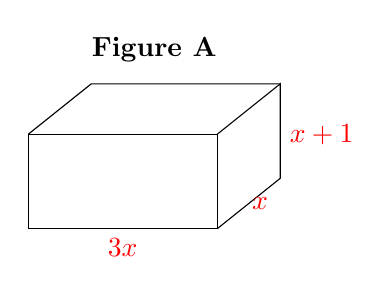
\begin{tikzpicture}[scale=0.8]
\draw (0,0) -- (3,0) node[midway, below, red] {\(3x\)} -- (3,1.5) -- (0,1.5) -- cycle;
\draw (3,0) -- (4,0.8) node[midway, right, red, inner sep=1pt] {\(x\)} -- (4,2.3) -- (3,1.5);
\draw (0,1.5) -- (1,2.3) -- (4,2.3);
\node[right, red] at (4,1.5) {\(x+1\)};
\node[above] at (2,2.5) {\textbf{Figure A}};
\end{tikzpicture}
\qquad
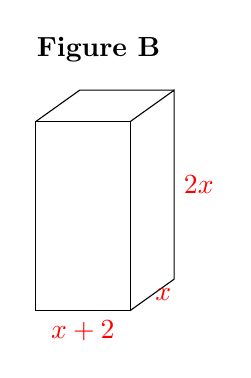
\begin{tikzpicture}[scale=0.8]
\draw (0,0) -- (1.5,0) node[midway, below, red] {\(x+2\)} -- (1.5,3) -- (0,3) -- cycle;
\draw (1.5,0) -- (2.2,0.5) node[midway, right, red, inner sep=1pt] {\(x\)} -- (2.2,3.5) -- (1.5,3);
\draw (0,3) -- (0.7,3.5) -- (2.2,3.5);
\node[right, red] at (2.2,2) {\(2x\)};
\node[above] at (1,3.8) {\textbf{Figure B}};
\end{tikzpicture}
\end{center}
}{}

\bankitem{Practice \#37 --- Modeling: interpret in context}{%
\textbf{Look for Relationships} A parallelogram with an area of \(\frac{3x + 12}{10x + 25}\) square units has a height shown. Find the length of the base of the parallelogram.

\begin{center}
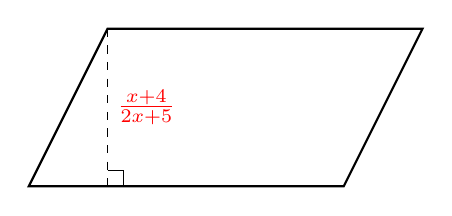
\begin{tikzpicture}
\draw[thick] (0,0) -- (4,0) -- (5,2) -- (1,2) -- cycle;
\draw[dashed] (1,2) -- (1,0);
\draw (1,0.2) -- (1.2,0.2) -- (1.2,0);
\node[right, red] at (1,1) {\(\frac{x + 4}{2x + 5}\)};
\end{tikzpicture}
\end{center}
}{}

\bankitem{Practice \#19 \IconStar\ ASSESSMENT CRITICAL --- Domain restrictions (LEHS Q\#2)}{%
\textbf{Reason} If the denominator of a rational expression is \(x^3 + 3x^2 - 10x\), what value(s) must be restricted from the domain for \(x\)?
}{}

\sectionbanner{SHARE / SUMMARY (5 min)}

\begin{sentenceframebox}
\textbf{Sentence frames}

Pair share (\#19): ``This ratio compares \_\_\_ to \_\_\_. The rational model is \_\_\_ / \_\_\_. After factoring and canceling, it simplifies to \_\_\_ with \(x \neq\) \_\_\_, which means in context that \_\_\_.''

Whole class: one pair reads \#19. Class signals thumbs up/sideways.
\end{sentenceframebox}

\begin{callout}{\IconChart\ CONCEPT SUMMARY (your reference for Topic 4 assessment)}{calloutell}
SIMPLIFYING RATIONAL EXPRESSIONS:\\
\hspace*{1.5em}--- FACTOR numerator and denominator completely.\\
\hspace*{1.5em}--- DOMAIN: exclude ALL zeros of any denominator (original AND intermediate steps).\\
\hspace*{1.5em}--- CANCEL common factors (they still exclude their zeros from the domain).\\
\hspace*{1.5em}--- Write simplified form WITH restriction: e.g., \(-(x+2)/(x+5)\), \(x \neq 2\), \(x \neq -5\).

\medskip
MODELING WITH RATIONAL EXPRESSIONS:\\
\hspace*{1.5em}--- Name the ratio in words first.\\
\hspace*{1.5em}--- Build each quantity as a polynomial, form the fraction, then simplify.\\
\hspace*{1.5em}--- Interpret the simplified ratio: what do the numerator and denominator mean?\\
\hspace*{1.5em}--- State domain restriction in context (e.g., ``\(x > 0\) because length is positive'').
\end{callout}

\sectionbanner{EXIT}

\begin{summaryexitbox}{EXIT TICKET --- Pre-Assessment Confidence Check}
A rational model needs factoring because \_\_\_.

My simplified ratio is \_\_\_, valid when \(x \neq\) \_\_\_.

In context this means \_\_\_.

One biggest thing I learned today: \_\_\_\_\_\_\_\_\_\_\_\_\_\_\_\_\_\_\_\_\_\_\_\_
\end{summaryexitbox}

\clearpage

\sectionbanner{OPTIONAL REINFORCEMENT (not collected)}
\textit{Extra stretch for fast finishers. Try without a calculator first.}

\bankitem{Optional \#1  (Savvas SAT/ACT style)}{%
\textbf{SAT/ACT} For what value of \(x\) is \(\frac{2x^2 + 8x}{(x + 4)(x^2 - 9)}\) undefined?
}{%
  \answerchoice{A}{\(-8\)}
  \answerchoice{B}{\(-3\)}
  \answerchoice{C}{\(0\)}
  \answerchoice{D}{\(4\)}
  \answerchoice{E}{\(9\)}
}

\end{document}
